\section{Method}\label{sec:method}

Based on the analysis in Sec. \ref{sec:background}, we introduce a control system that consists of two parts. The first part is based on conventional feedback control theory and maximize all reward terms that are functions of $s_\text{m}$. An RL method is superposed and maximizes the reward terms that are functions of $s_\text{o}$.

\subsection{Residual Reinforcement Learning}
In most robotics tasks, we consider rewards of the form:
%
\begin{equation}\label{eq:reward}
    r_t = f(s_\text{m}) + g(s_\text{o}).
\end{equation}
%
The term $f(s_\text{m})$ is assumed to be a function, which represents a geometric relationship of robot states, such as a Euclidean distance or a desired trajectory.
%% AVN is this a necessary assumption?
The second term of the sum $g(s_\text{o})$ can be a general class of functions. Concretely, in our model assembly task, $f(s_m)$ is the reward for moving the robot gripper between the standing blocks, while $g(s_o)$ is the reward for keeping the standing blocks upright and in their original positions.

The key insight of residual RL is that in many tasks, $f(s_\text{m})$ can be easily optimized a priori of any environment interaction by conventional controllers, while $g(s_\text{o})$ may be easier to learn with RL which can learn fine-grained hand-engineered feedback controllers even with friction and contacts.
To take advantage of the efficiency of conventional controllers but also the flexbility of RL, we choose:
%
\begin{equation}\label{eq:ctrl_seq}
    u = \pi_H(s_\text{m}) + \pi_\theta(s_\text{m}, s_\text{o})
\end{equation}
%
as the control action, where $\pi_H(s_\text{m})$ is the human-designed controller and $\pi_\theta(s_\text{m}, s_\text{o})$ is a learned policy parametrized by $\theta$ and optimized by an RL algorithm to maximize expected returns on the task.

Inserting \eqref{eq:ctrl_seq} into \eqref{eq:eom} one can see that a properly designed feedback control law for $\pi_H(s_\text{m})$ is able to provide exponentially stable error dynamics of $s_\text{m}$ if the learned controller $\pi_\theta$ is neglected and the sub statespace is stabilizable.
This is equivalent to maximizing \eqref{eq:reward} for the case $f$ represents errors between actual and desired states.

The residual controller $\pi_\theta(s_\text{m}, s_\text{o})$ can now be used to maximize the reward term $g(s_\text{o})$ in \eqref{eq:reward}.
Since the control sequence \eqref{eq:ctrl_seq} enters \eqref{eq:eom} through the dynamics of $s_\text{m}$ and $s_\text{m}$ is in fact the control input to the dynamics of $s_\text{o}$, we cannot simply use the a-priori hand-engineered feedback controller to achieve zero error of $s_\text{m}$ and independently achieve the control objective on $s_\text{o}$.
Through the coupling of states we need to perform an overall optimization of \eqref{eq:ctrl_seq}, whereby the hand-engineered feedback controller provides internal structures and eases the optimization related to the reward term $f(s_\text{m})$.

\setlength{\textfloatsep}{0.09cm}
\begin{algorithm}
   	\caption{Residual reinforcement learning}
   	\label{alg:residualrl}
   	\begin{algorithmic}[1]
    \REQUIRE policy $\pi_\theta$, hand-engineered controller $\pi_\text{H}$.
    \FOR{$n=0,...,N-1$ episodes}
        \STATE Initialize random process $\mathcal{N}$ for exploration
        \STATE Sample initial state $s_0 \sim E$.
        \FOR{$t=0,...,H -1$ steps}
            \STATE Get policy action $u_t = \pi_\theta(s_t) + \mathcal{N}_t$.
            \STATE Get action to execute $u'_t = u_t + \pi_\text{H}(s_t)$.
            \STATE Get next state $s_{t+1} \sim p(\cdot \mid s_t, u'_t)$.
            \STATE Store $(s_t, u_t, s_{t+1})$ into replay buffer $\mathcal R$.
            \STATE Sample set of transitions $(s, u, s') \sim \mathcal R$.
            \STATE Optimize $\theta$ using RL with sampled transitions.
        \ENDFOR
    \ENDFOR
   	\end{algorithmic}
\end{algorithm}
\setlength{\floatsep}{0.09cm}
\subsection{Method Summary}
Our method is summarized in Algorithm \ref{alg:residualrl}. The key idea is to combine the flexibility of RL with the efficiency of conventional controllers by additively combining a learnable parametrized policy with a fixed hand-engineered controller.

\begin{figure*}[t]
    \vspace{6pt}
    \centering
    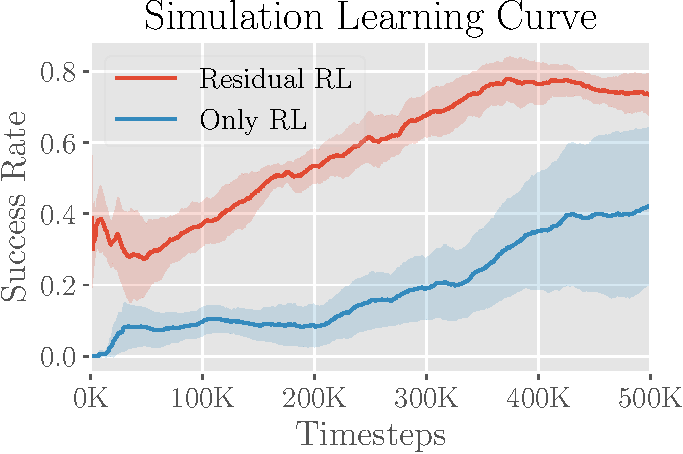
\includegraphics[height=1.1in]{residualrl/figs/sim_learning_curve3.pdf}
    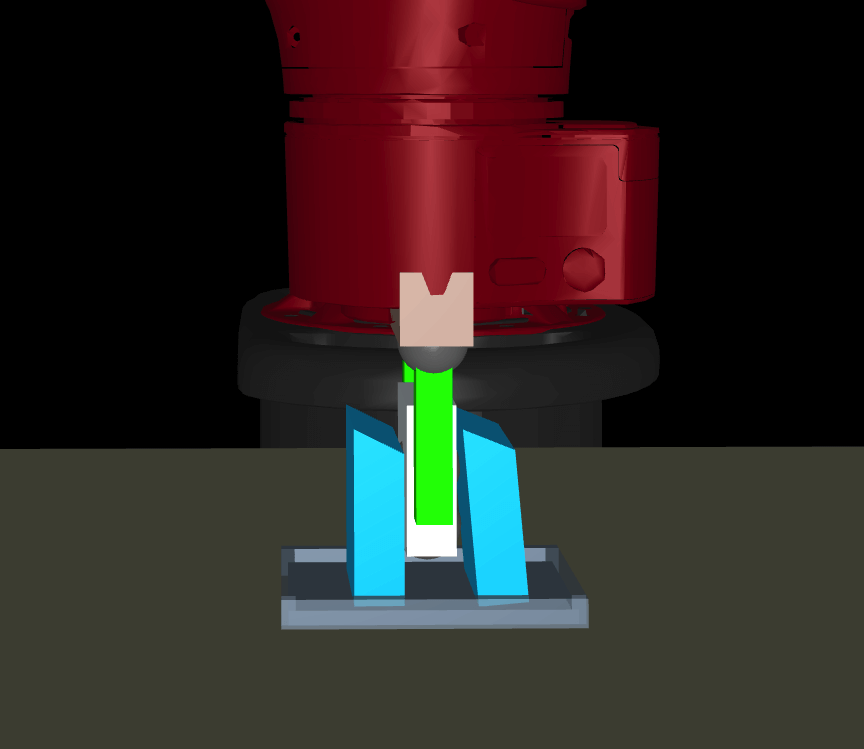
\includegraphics[height=1.1in]{residualrl/figs/sawyer_env.png} 
    \hspace{.1cm}
    
\includegraphics[height=1.1in]{residualrl/figs/real_world_env.png} 
    \vspace{0.1cm}
    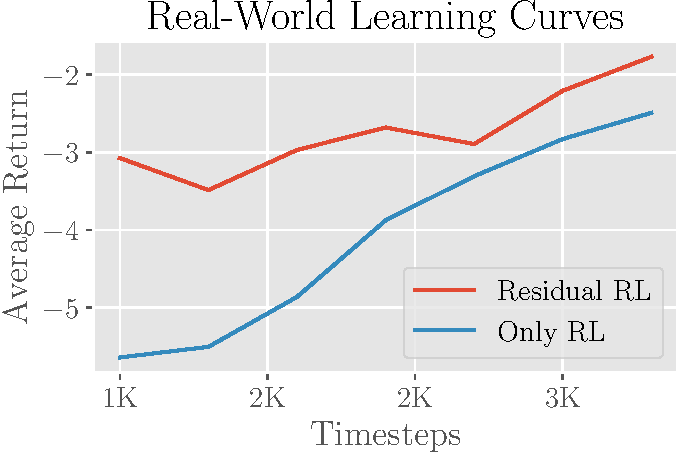
\includegraphics[height=1.1in]{residualrl/figs/real_residualrl_comparison.pdf}
    \caption{Block assembly task in simulation (left) and  real-world (right). The task is to insert a block between the two blocks on the table without moving the blocks or tipping them over. In the learning curves, we compare our method with RL without any hand-engineered controller\protect\footnotemark. In both simulation and real-world experiments, we see that residual RL learns faster than RL alone, while achieving better performance than the hand-engineered controller. }%
    \label{fig:fig2}
\end{figure*}

As our underlying RL algorithm, we use a variant of twin delayed deep deterministic policy gradients (TD3)
as described in~\cite{fujimoto2018td3}. TD3 is a value-based RL algorithm for continuous control based off of the deep deterministic policy gradient (DDPG) algorithm \cite{lillicrap2015continuous}. We have found that TD3 is stable, sample-efficient, and requires little manual tuning compared to DDPG.
We used the publicly available \href{https://github.com/vitchyr/rlkit}{\texttt{rlkit}} implementation of TD3 \cite{pong2018tdm}. Our method is independent of the choice of RL algorithm, and we could apply residual RL to any other RL algorithm.